Con il termine \textit{Biologia Computazionale} si intende la scienza che si prefigge l'obiettivo di sviluppare e applicare algoritmi, modelli e metodi matematici al fine di studiare sistemi biologici \cite{Searls19983}. E' una scienza interdisciplinare che attinge a conoscenze di altri campi come matematica, biologia, statistica, biochimica al fine di perseguire i propri obiettivi \cite{AbouttheCCMB}.

Lo sviluppo della biologia computazionale iniziò negli anni 70 del secolo scorso, da allora una sempre più grande mole di dati e una modesta quantità di pubblicazioni in questo campo, hanno contribuito a rendere questa scienza quella che è oggi.

\section{Obiettivi}
Approcci studiati dalla biologia computazionale sonostati utilizzati per portare a termine vari compiti, tra cui il sequenziamento del genoma umano, creare modelli accurati del cervello umano e dei sistemi biologici.

Alcune sfide che si prefigge la biologia computazionale sono \cite{Searls19983}: 

\begin{itemize}
    \item \textsc{Analisi Struttura delle Proteine.} Capire quali sono le proteine presenti in un campione biologico.
    \item \textsc{Ricerca di omologie nelle sequenze genomiche}
    \item \textsc{Allineamento multiplo di sequenze e ricostruzione di filogenesi.} Analizzare la storia evolutiva di più specie.
    \item \textsc{Analisi di Sequenze.} Comparazione di sequenze genomiche di specie similari o distinte al fine di evidenziare omologie e differenze. Ricostruzione di lunghe sequenze genomiche a partire da frammenti. Correzione di errori da parte delle macchine sequenziatrici. 
\end{itemize}

\section{Bioinformatica}
In particolare la \textit{Bioinformatica} si focalizza sullo studio di tecniche ed algoritmi per l'analisi di strighe (sequenze), applicando e studiando metodi tipici delle scienze informatiche, creando quindi interdisciplinarietà tra le due materie.


Alcuni esempi delle tecniche studiate in Bioinformatica sono:

\begin{itemize}
    \item \textsc{Pattern Recognition.} Identificare una sottostringa all'interno di una più estesa.
        \begin{figure}[h]
        \centering
        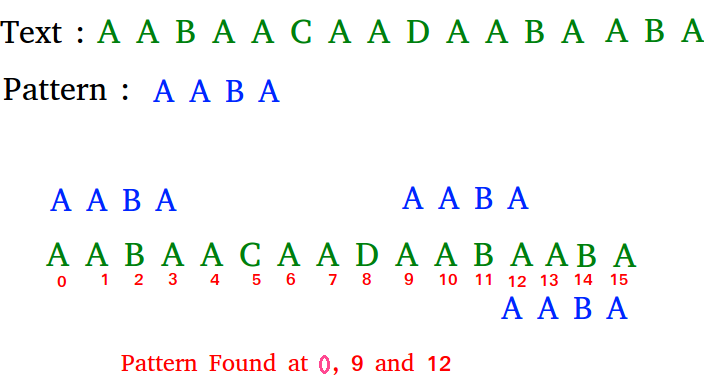
\includegraphics[scale= 0.5]{images/pattern matching.png}
        \caption{Esempio grafico di pattern matching}
        \label{fig:pattern_matching}
        \end{figure}
    \item \textsc{Data Mining}
    \item \textsc{Machine Learning Algorithms}
\end{itemize}

E' da notare che, in realtà, il termine \textit{Bioinformatica} è usato per evidenziare una più ampia gamma di studi inerenti alla biologia che utilizzano approcci informatici per portare a temine i propri obiettivi.

\newpage

\section{Introduzione alla Biologia e Terminologia}
Questa Relazione ha lo scopo di esporre il problema affrontato durante lo stage del terzo anno da un punto di vista informatico. Nonostante ciò verrà fatta un'introduzione ai concetti necessari di biologia molecolare, in modo da facilitare la comprensione di quanto segue.

In biologia Molecolare, la \textit{Trascrizione} è un processo mediante il quale il le informazioni contenute nel Dna vengo trascritte su una molecola di Rna.
Un \textit{gene} è una regione del genoma (detta \textit{locus}) che esprime una proteina e viene identificato attraverso il suo \textit{Hugo name} che è un acronimo della sua descrizione.

Si può pensare ad un gene come un'alternanza di regioni codificanti (esoni) e regioni non codificanti (introni).

\begin{figure}[ht]
    \centering
    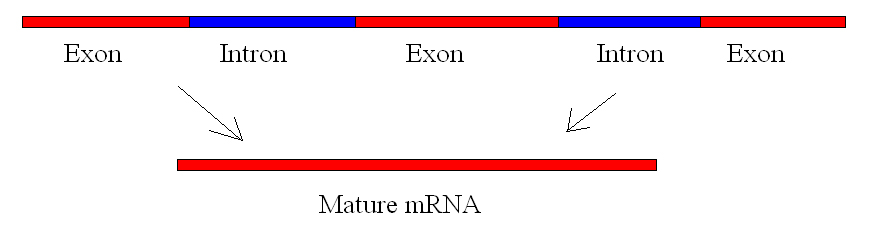
\includegraphics[scale=0.3]{images/introns - exons.jpg}
    \caption{Alternanza di introni ed Esoni}
    \label{fig:intron-exon}
\end{figure}

Il confine tra esone ed introne è detto \textit{Splicing site al 5'}, mentre il confine tra introne ed esone è detto \textit{Splicing site al 3'}.

Quando avviene una \textit{Trascrizione}, il locus del gene viene copiato, compiendo una sostituzione tra le molecole di \textit{Timina} e \textit{Uracile}. Dal punto di vista informatico, il locus è una stringa su alfabeto \textbf{A, C, G, T}, dopo la trascrizione, l'alfabeto diventa \textbf{A, C, G, U} e la molecola formata prende il nome di \newline \textit{pre - mRna}. Successivamente vengono eliminate le regioni non codificanti e viene formata la molecola di \textit{mRna} (trascritto).

%\newpage

I geni umani sono circa 25000, invece le proteine sono centinaia di migliaia. La corrispondenza 1:1 non è rispettata in quanto un gene può ricombinare i sui esoni in modi diversi al fine di esprimere una molteplicità di trascritti (quindi proteine).
Tutti i trascritti del gene vengono dette \textit{Isoforme di Splicing} del gene.  

\begin{figure}[ht]
    \centering
    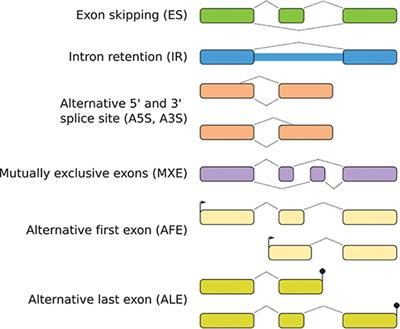
\includegraphics[scale=0.6]{images/alternative splicing.jpg}
    \caption{Esempi di Isoforme di Spliging}
    \label{fig:slicing}
\end{figure}

Studi recenti asseriscono che lo splicing alternativo avvenga sul 90\% dei geni di Homo Sapiens.

Uno dei motivi per cui è utile studiare le isoforme di splicing di un gene è quello che sono fortemente legate alle malattie.

Patten frequenti dell'alternative splicing sono Exon skiping, Intron Retention, 5' Competing Site, 3' Competing Site, Multiple promoters.

